\chapter{Parameter-efficient Fine-Tuning (PEFT)}





\section{Modern LLM Fine-Tuning}

Recent years have witnessed an unprecedented growth in the size of Large Language Models (LLMs). Early neural language models contained only millions of parameters, whereas modern foundation models contain billions or even hundreds of billions of parameters. These models acquire extensive knowledge during large-scale pretraining, enabling them to perform a wide range of downstream tasks such as question answering, summarization, translation, reasoning, and code generation.

However, pretrained LLMs are general-purpose models. To specialize an LLM for a particular application (e.g., medicine, finance, or law), it must be adapted using task-specific data. Traditionally, this adaptation is achieved through \textbf{full fine-tuning}, in which every trainable parameter of the pretrained model is updated.
\subsection*{Why Can't We Fully Fine-Tune Large LLMs?}

The traditional fine-tuning pipeline is illustrated below:

\[
\text{Pretraining}
\longrightarrow
\text{Pretrained Model}
\longrightarrow
\text{Full Fine-Tuning}
\longrightarrow
\text{Task-Specific Model}
\]

During full fine-tuning, gradients are computed for every trainable layer, and every parameter of the model is updated using the downstream dataset.

For relatively small neural networks, updating all parameters is computationally feasible. However, modern LLMs contain billions of parameters, making full fine-tuning increasingly expensive in terms of both memory consumption and computational cost.
\begin{table}[H]
\centering
\caption{Parameter scale of representative modern Large Language Models.}
\label{tab:llm_parameters}

\renewcommand{\arraystretch}{1.25}

\begin{tabular}{lc}
\toprule
\textbf{Model} & \textbf{Parameters} \\
\midrule
Llama 3 8B  & 8 Billion \\
Llama 3 70B & 70 Billion \\
Qwen 72B    & 72 Billion \\
\bottomrule
\end{tabular}

\end{table}
Updating billions of parameters during every training step is fundamentally different from training conventional neural networks.

Training such large models requires substantially more GPU memory than simply storing the model weights. During optimization, additional information must also be maintained, including:

\begin{itemize}
    \item Model parameters;
    \item Gradients;
    \item Optimizer states;
    \item Intermediate activations.
\end{itemize}

Consequently, memory consumption grows rapidly as the number of trainable parameters increases.

Most modern LLMs are optimized using the AdamW optimizer. Unlike standard stochastic gradient descent, AdamW maintains additional statistics for every trainable parameter:

\begin{itemize}
    \item Parameter value;
    \item First moment estimate ($m$);
    \item Second moment estimate ($v$).
\end{itemize}

Therefore, each trainable parameter requires considerably more memory than its weight alone.
In addition to memory consumption, full fine-tuning is computationally expensive because every optimization step must perform

\[
\text{Forward Pass}
\longrightarrow
\text{Backward Pass}
\longrightarrow
\text{Parameter Update}
\]

for billions of trainable parameters.

As model size increases, training becomes progressively slower and requires increasingly powerful hardware.

\subsection*{Do We Really Need to Update Everything?}

Although modern LLMs already possess extensive knowledge acquired during pretraining, full fine-tuning updates every parameter regardless of whether that knowledge is relevant to the downstream task.

For example, when adapting an LLM into a medical assistant, much of its existing linguistic ability, reasoning capability, and general world knowledge remains useful. Only a relatively small amount of new task-specific knowledge must be learned.

This observation raises an important question:

\begin{center}
\emph{Is it really necessary to update billions of parameters to learn a new task?}
\end{center}

The answer is often \textbf{no}. Instead of modifying the entire model, it is possible to freeze the pretrained model and train only a small number of additional parameters while preserving the knowledge acquired during pretraining.

This idea forms the foundation of \textbf{Parameter-Efficient Fine-Tuning (PEFT)}, which dramatically reduces memory usage and computational cost while maintaining competitive performance.
\clearpage
\section{Parameter-Efficient Fine-Tuning (PEFT)}

Parameter-Efficient Fine-Tuning (PEFT) is not a single algorithm but rather a family of fine-tuning methods that share the same fundamental philosophy. Instead of updating every parameter of a pretrained Large Language Model, PEFT freezes the original model and trains only a small number of additional parameters.

The two core principles of PEFT are:

\begin{itemize}
    \item \textbf{Freeze the pretrained model:} The original LLM remains unchanged throughout training, preserving the knowledge acquired during large-scale pretraining.
    \item \textbf{Train a small set of additional parameters:} Only lightweight modules are optimized to learn the task-specific adaptation.
\end{itemize}

Conceptually, the pretrained model provides the general knowledge required for language understanding and reasoning, while the newly introduced trainable parameters learn how to adapt that knowledge to a particular downstream task.

\begin{figure}[H]
\centering
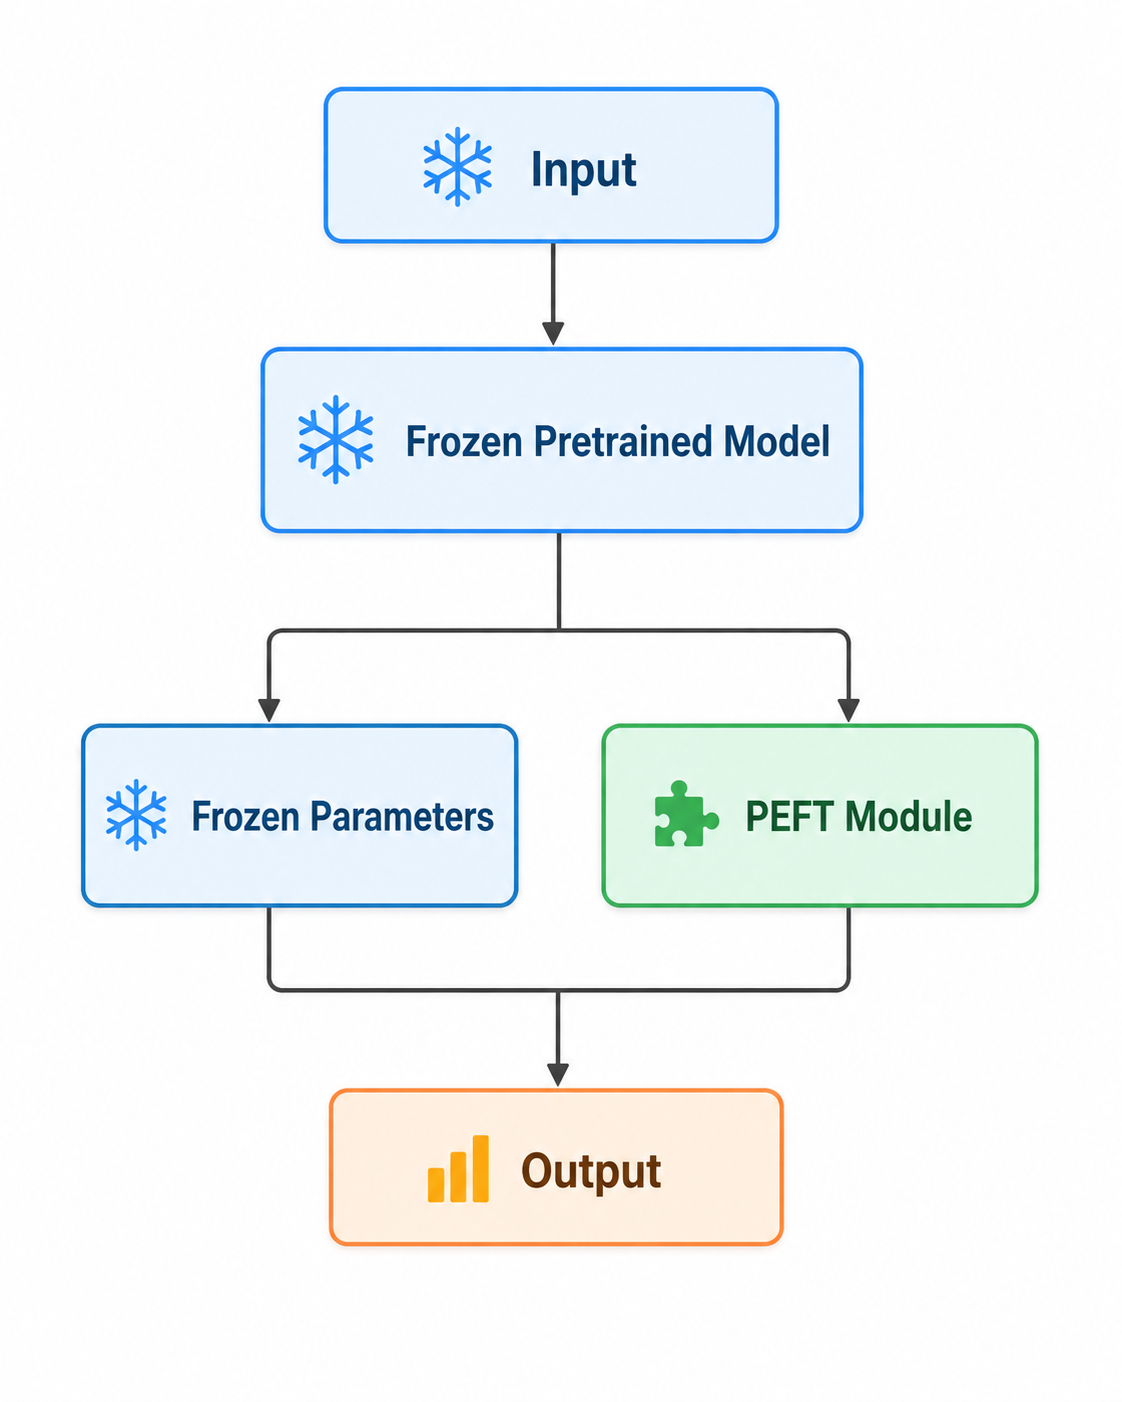
\includegraphics[width=0.95\textwidth]{figures/12-1 figure.png}
\label{fig:peft_transition_ch12}
\end{figure}

Rather than replacing the pretrained knowledge, the trainable module complements it by learning only the additional information required for the target task. Consequently, PEFT significantly reduces the number of trainable parameters, GPU memory consumption, and training time while achieving performance that is often comparable to full fine-tuning.

\section{Main PEFT Methods}

Before the introduction of LoRA, several Parameter-Efficient Fine-Tuning (PEFT) techniques had already been proposed to reduce the number of trainable parameters while preserving the knowledge contained in pretrained Large Language Models. Although these methods differ in their implementation, they all share the same objective: to adapt a frozen pretrained model by training only a small set of additional parameters.

The most representative approaches are Adapter Tuning, Prompt Tuning, and Prefix Tuning.
\subsection*{Adapter Tuning}

Adapter Tuning introduces small trainable neural networks, called \emph{adapters}, into each Transformer layer. During fine-tuning, the original model parameters remain frozen, and only the adapter modules are optimized.

A typical adapter consists of a bottleneck multilayer perceptron (MLP). The hidden representation is first projected into a lower-dimensional space and then projected back to its original dimension. For example,

\[
4096
\longrightarrow
64
\longrightarrow
4096
\]

This bottleneck architecture greatly reduces the number of trainable parameters while allowing the model to learn task-specific representations.

The overall computation can be summarized as

\[
\text{Transformer Layer}
\longrightarrow
\text{Adapter}
\longrightarrow
\text{Transformer Layer}.
\]

Because only the adapter parameters are updated, Adapter Tuning significantly reduces GPU memory consumption compared with full fine-tuning.
\subsection*{Prompt Tuning}

Prompt Tuning follows a different strategy. Instead of inserting additional neural network layers, it keeps the entire pretrained model frozen and learns only a small number of trainable embedding vectors called \emph{soft prompts}.

Consider the input sentence

\[
\texttt{Translate to French: Hello}
\]

Normally, each token is converted into an embedding vector before entering the Transformer.

Prompt Tuning prepends several trainable vectors to the input sequence:

\[
P_1,\;
P_2,\;
P_3,\;
e_1,\;
e_2,\;
e_3,\;
e_4,\;
e_5
\]

where

\begin{itemize}
\item $P_1,P_2,P_3$ are trainable prompt embeddings;
\item $e_1,\ldots,e_5$ are the original token embeddings.
\end{itemize}
\begin{figure}[H]
\centering
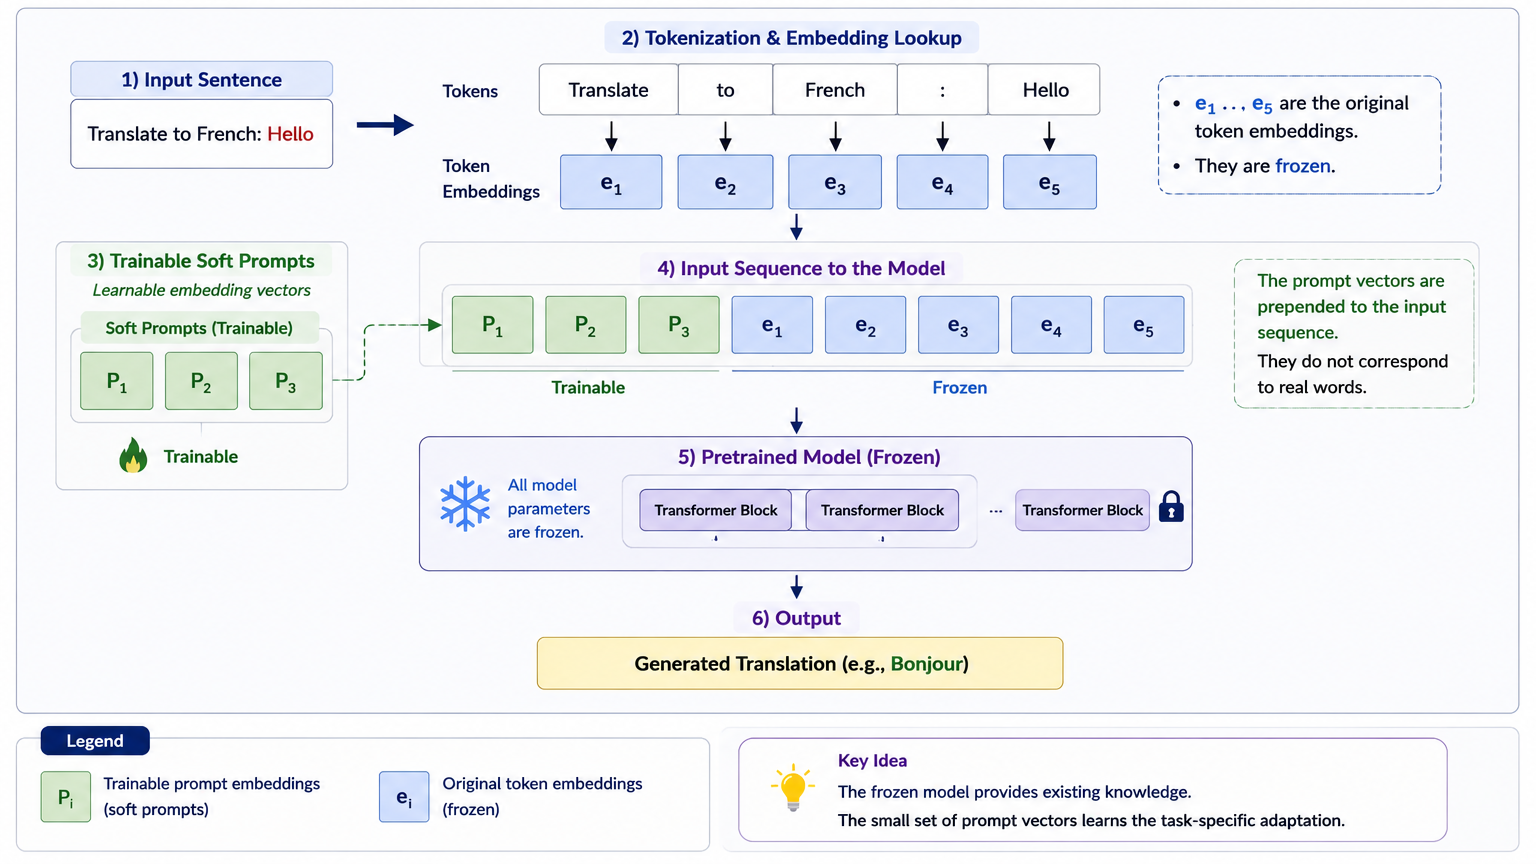
\includegraphics[width=0.95\textwidth]{figures/12-6 figure.png}
\end{figure}
Unlike ordinary tokens, the prompt vectors do not correspond to actual words. They are simply learnable vectors with the same dimensionality as the token embeddings.

During training,

\begin{itemize}
\item the Transformer parameters remain frozen;
\item only the prompt embeddings are updated using gradient descent.
\end{itemize}
\clearpage 
\begin{figure}[H]
\centering
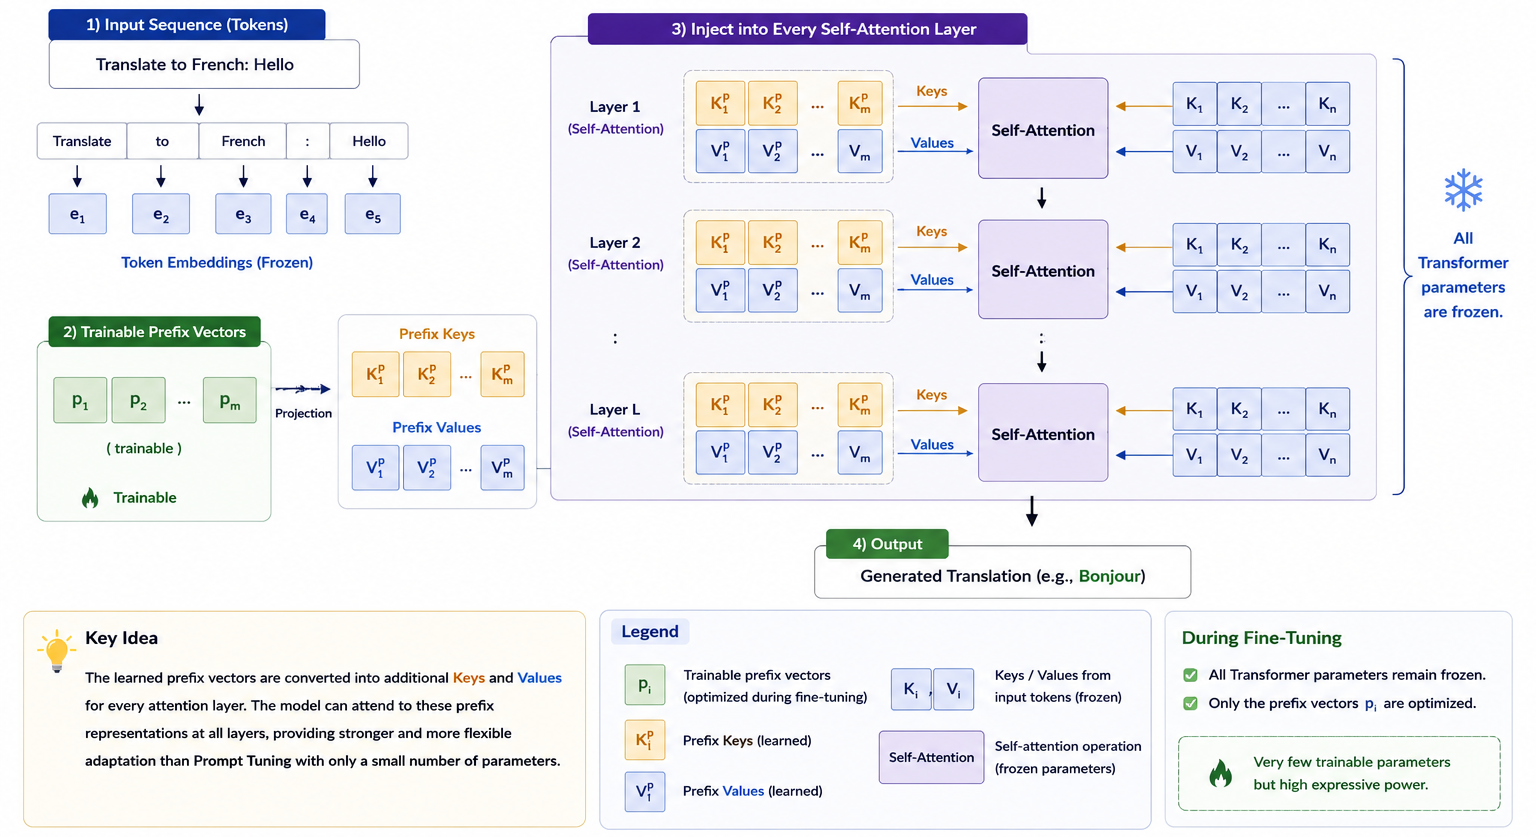
\includegraphics[width=0.95\textwidth]{figures/12-7 figure.png}
\end{figure}
Over time, these learned prompt vectors steer the pretrained model toward the desired downstream task without modifying its original parameters.
\subsection*{Prefix Tuning}

Prefix Tuning extends the idea of Prompt Tuning by injecting trainable vectors directly into the Transformer's attention mechanism rather than into the input sequence.

Instead of learning additional input embeddings, Prefix Tuning learns a set of trainable prefix vectors that are transformed into additional \textbf{Keys} and \textbf{Values} for every self-attention layer.

Consequently, each attention layer attends not only to the original input tokens but also to the learned prefix representations.

The computation can be summarized as

\[
\text{Trainable Prefix}
\longrightarrow
(K_{\text{prefix}},V_{\text{prefix}})
\longrightarrow
\text{Self-Attention}
\longrightarrow
\text{Output}.
\]

During fine-tuning,

\begin{itemize}
\item all Transformer parameters remain frozen;
\item only the prefix vectors are optimized.
\end{itemize}

Because the learned prefixes influence every attention layer, Prefix Tuning generally provides greater expressive power than Prompt Tuning while still requiring only a very small number of trainable parameters.


\section{LoRA (Low-Rank Adaptation)}

Large Language Models contain numerous weight matrices within their Transformer layers, such as the projection matrices used to compute queries, keys, values, and feed-forward transformations. During conventional full fine-tuning, every weight matrix is updated using task-specific data.

If a pretrained weight matrix is denoted by \(W\), the updated weights can be written as

\[
W' = W + \Delta W,
\]

where

\begin{itemize}
    \item \(W\) denotes the pretrained weight matrix;
    \item \(\Delta W\) is the trainable weight update learned during fine-tuning.
\end{itemize}

The main limitation of full fine-tuning is that the update matrix \(\Delta W\) has exactly the same dimensions as \(W\). Consequently, if \(W\) contains millions of parameters, then \(\Delta W\) also introduces millions of additional trainable parameters.

Researchers observed that although the weight matrices are very large, the learned updates often possess a much lower intrinsic rank. In other words, the model does not require millions of completely independent parameter updates. Instead, most of the useful task-specific information can be represented within a much smaller low-dimensional subspace.

This observation forms the key idea behind \textbf{Low-Rank Adaptation (LoRA)}.
\subsection*{Low-Rank Approximation}

Instead of learning the full update matrix \(\Delta W\), LoRA approximates it as the product of two much smaller matrices:

\[
\boxed{\Delta W = BA}
\]

where

\[
A \in \mathbb{R}^{r\times d},
\qquad
B \in \mathbb{R}^{k\times r},
\]

and

\[
r \ll d,\; k.
\]

The value \(r\) is called the \textbf{rank} of the LoRA decomposition and is typically chosen from

\[
r \in \{4,\,8,\,16,\,32,\,64\}.
\]

Since \(r\) is much smaller than both \(d\) and \(k\), the number of trainable parameters is drastically reduced.

The term \emph{Low-Rank Adaptation} originates directly from this low-rank decomposition of the weight update.
\begin{figure}[H]
\centering
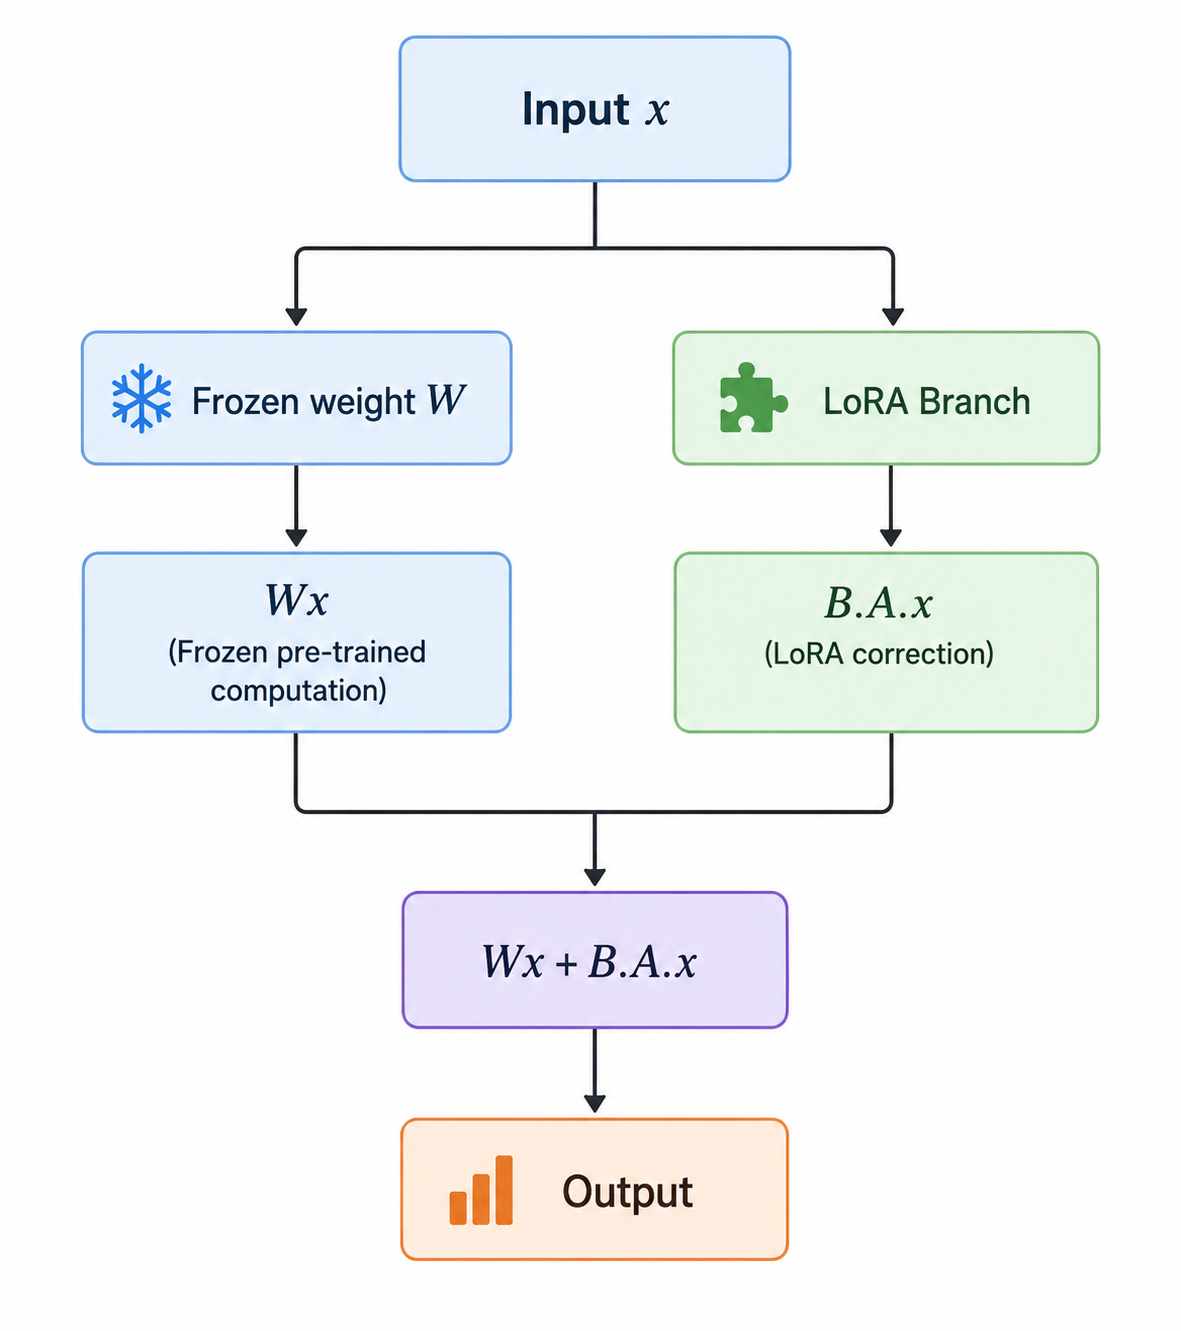
\includegraphics[width=0.9\textwidth]{figures/12-2 figure.png}
\label{fig:12-4}
\end{figure}
\subsection*{Numerical Example}

Suppose a pretrained weight matrix has dimensions

\[
W \in \mathbb{R}^{4096\times4096}.
\]

With full fine-tuning, the entire matrix must be updated, requiring

\[
4096 \times 4096
=
16.8\text{ million}
\]

trainable parameters.

Assume that LoRA uses a rank of

\[
r=8.
\]

Then only two small matrices are learned:

\[
A\in\mathbb{R}^{8\times4096},
\]

\[
B\in\mathbb{R}^{4096\times8}.
\]

Their product

\[
BA
=
(4096\times8)
(8\times4096)
=
4096\times4096
\]

has exactly the same dimensions as the original weight matrix and therefore can replace the full update \(\Delta W\).
\subsection*{Forward Pass}

During inference and training, the pretrained weight matrix remains frozen. The output is computed as

\[
y
=
Wx
+
BAx,
\]

where

\begin{itemize}
    \item \(Wx\) is the output produced by the frozen pretrained model;
    \item \(BAx\) is the low-rank correction learned by LoRA.
\end{itemize}

next Figure illustrates this computation, where the original branch remains frozen while the LoRA branch learns the task-specific adaptation.

\begin{figure}[H]
\centering
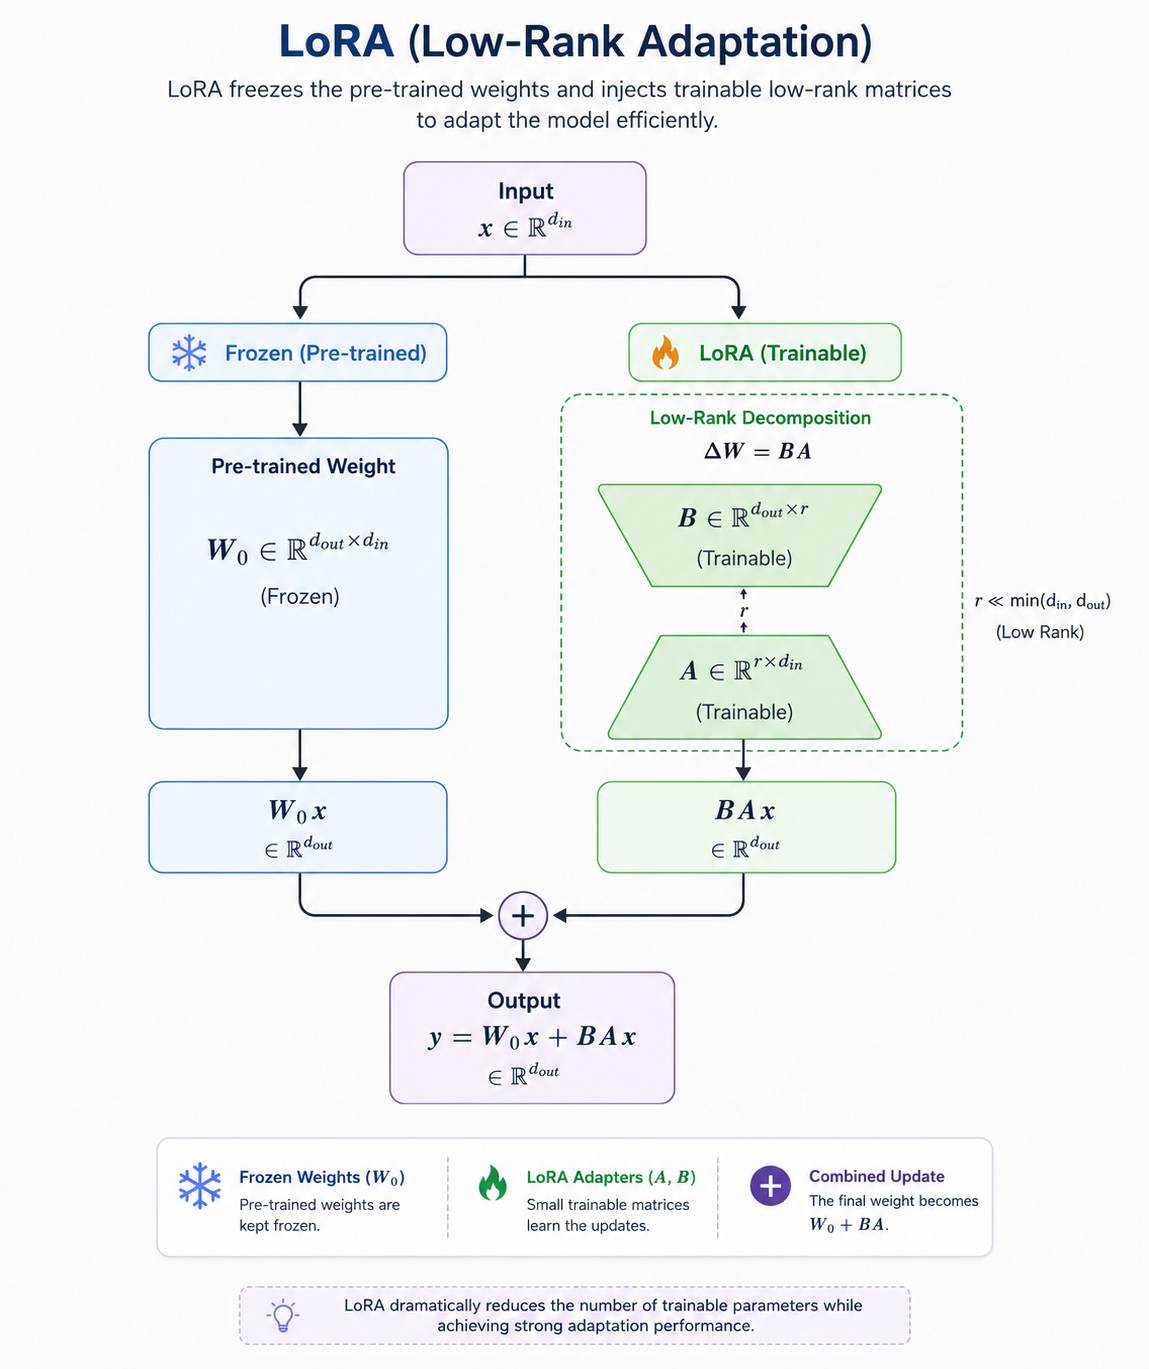
\includegraphics[width=0.85\textwidth]{figures/12-4 figure.png}
\label{fig:lora_architecture}
\end{figure}

\subsection*{Parameter Reduction}

Continuing the previous example,

\[
W
=
4096\times4096
=
16.8
\text{ million parameters}.
\]

LoRA learns only

\[
A:
8\times4096
=
32\,768,
\]

and

\[
B:
4096\times8
=
32\,768.
\]

Therefore, the total number of trainable parameters becomes

\[
32\,768
+
32\,768
=
65\,536
\approx
64\text{K}.
\]

Consequently, LoRA reduces the number of trainable parameters from approximately \(16.8\) million to only \(64\) thousand, corresponding to a reduction of more than \(250\times\).
\subsection*{Why Does LoRA Work?}

A pretrained Large Language Model already contains extensive knowledge acquired during large-scale pretraining, including language understanding, reasoning abilities, and factual information. For many downstream tasks, only a relatively small modification of the pretrained weights is required.

Instead of relearning the entire weight matrix, LoRA learns only this small task-specific correction through the low-rank update \(BA\). As a result, the pretrained knowledge is preserved while the model efficiently adapts to the new task using only a tiny fraction of the parameters required by full fine-tuning.
\subsection*{Transformer Weight Matrices}

A Transformer layer contains several trainable weight matrices distributed across its self-attention and feed-forward (MLP) components.

Within the self-attention mechanism, the input representation is projected into three different spaces using separate linear transformations:

\[
\text{Input}
\longrightarrow
W_Q,\;W_K,\;W_V
\longrightarrow
\text{Self-Attention}
\longrightarrow
W_O,
\]

where

\begin{itemize}
    \item $W_Q$ is the Query projection matrix;
    \item $W_K$ is the Key projection matrix;
    \item $W_V$ is the Value projection matrix;
    \item $W_O$ is the Output projection matrix.
\end{itemize}

In addition to the attention mechanism, every Transformer layer contains a feed-forward network (MLP), which is composed of two linear transformations separated by a nonlinear activation function:

\[
\text{Input}
\longrightarrow
\text{Linear}
\longrightarrow
\text{Activation}
\longrightarrow
\text{Linear}
\longrightarrow
\text{Output}.
\]

Each linear transformation in both the attention module and the MLP possesses its own trainable weight matrix.


\subsection*{Where Can We Apply LoRA?}

Since LoRA modifies only linear transformations, it can theoretically be attached to any weight matrix inside a Transformer layer.

Possible insertion points include

\[
W_Q,\;
W_K,\;
W_V,\;
W_O,
\]

as well as the two linear layers of the MLP.

When LoRA is applied to a weight matrix, the original transformation

\[
W
\]

is replaced by

\[
W + BA,
\]

where the pretrained matrix $W$ remains frozen and only the low-rank matrices $A$ and $B$ are optimized.

Suppose a Transformer contains one hundred linear layers. Applying LoRA to every layer would still require significantly fewer trainable parameters than full fine-tuning. Nevertheless, doing so would increase

\begin{itemize}
    \item the number of trainable parameters;
    \item GPU memory consumption;
    \item training time.
\end{itemize}

Consequently, an important design choice is determining which weight matrices should receive LoRA modules.
\subsection*{Which Layers Are Usually Chosen?}

Empirical studies have shown that not all weight matrices contribute equally to downstream adaptation.

For many modern Large Language Models, LoRA is commonly applied only to the Query and Value projection matrices:

\[
W_Q
\quad\text{and}\quad
W_V.
\]

These matrices directly influence the attention mechanism by determining how tokens attend to one another. Modifying only the Query and Value projections allows the model to learn new attention patterns while leaving the majority of the pretrained network unchanged.

Although LoRA can also be applied to the Key, Output, and MLP projection matrices, restricting the adaptation to $W_Q$ and $W_V$ often provides an excellent trade-off between computational efficiency and downstream performance. Consequently, this configuration has become the default choice in many practical implementations of LoRA.
\begin{table}[H]
\centering
\caption{Common insertion points for LoRA in a Transformer layer.}
\label{tab:lora_layers}

\renewcommand{\arraystretch}{1.3}

\begin{tabular}{ll}
\toprule
\textbf{Layer} & \textbf{Commonly Used} \\
\midrule
Query Projection ($W_Q$) & \checkmark \\
Key Projection ($W_K$) & Optional \\
Value Projection ($W_V$) & \checkmark \\
Output Projection ($W_O$) & Optional \\
MLP Linear Layer 1 & Optional \\
MLP Linear Layer 2 & Optional \\
\bottomrule
\end{tabular}

\end{table}

\subsection*{Why Is LoRA Usually Applied to Query and Value?}

Although LoRA can theoretically be applied to any linear layer in a Transformer, empirical studies have shown that some weight matrices contribute more than others to downstream adaptation.

The Query projection matrix ($W_Q$) determines how each token searches for relevant information, while the Value projection matrix ($W_V$) controls the information that is ultimately transmitted through the attention mechanism. Adapting these two matrices allows the model to learn new attention behaviors with relatively few trainable parameters.

In contrast, the Key projection matrix ($W_K$) defines how tokens are matched during attention. In many experiments, updating $W_K$ provides only modest performance improvements while increasing the computational cost. Consequently, many practical implementations omit LoRA on the Key projection.

For more challenging tasks, some implementations also apply LoRA to the Output projection ($W_O$) or even to the feed-forward (MLP) layers.

Typical LoRA configurations include

\[
W_Q + W_V,
\]

\[
W_Q + W_K + W_V,
\]

\[
W_Q + W_V + W_O,
\]

or

\[
\text{All Linear Layers}.
\]

The choice depends on several factors:

\begin{itemize}
    \item available GPU memory;
    \item task complexity;
    \item desired accuracy.
\end{itemize}
\subsection*{Typical Configurations in Modern LLMs}

Many popular Large Language Models apply LoRA primarily to the Query and Value projection matrices. Examples include

\begin{center}
\renewcommand{\arraystretch}{1.2}
\begin{tabular}{ll}
\toprule
\textbf{Model Family} & \textbf{Typical LoRA Targets} \\
\midrule
Llama & $W_Q,\;W_V$ \\
Mistral & $W_Q,\;W_V$ \\
Gemma & $W_Q,\;W_V$ \\
Phi & $W_Q,\;W_V$ \\
Qwen & $W_Q,\;W_V$ (sometimes all linear layers) \\
\bottomrule
\end{tabular}
\end{center}

More recent implementations often apply LoRA to all linear layers of the Transformer. Although this slightly increases the number of trainable parameters, it generally provides better downstream performance while remaining far more efficient than full fine-tuning.
\subsection*{LoRA Scaling Factor}

Besides the rank $r$, another important hyperparameter is the scaling factor, denoted by $\alpha$.

Rather than computing the update simply as

\[
W + BA,
\]

LoRA actually applies

\[
W+\frac{\alpha}{r}BA.
\]

The factor

\[
\frac{\alpha}{r}
\]

controls the contribution of the LoRA update relative to the frozen pretrained weights.

Intuitively, a larger value of $\alpha$ increases the influence of the learned adaptation, whereas a smaller value keeps the model closer to the original pretrained parameters.

Typical values are

\[
\alpha \in [16,\,64].
\]
\subsection*{LoRA Dropout}

Many LoRA implementations optionally apply dropout to the LoRA branch during training.

The objective is to

\begin{itemize}
    \item reduce overfitting;
    \item improve generalization;
    \item increase robustness, particularly when fine-tuning on small datasets.
\end{itemize}

Typical dropout values range from

\[
0.0
\quad\text{to}\quad
0.1.
\]
\section{Training with LoRA}

During LoRA fine-tuning, the pretrained Transformer remains completely frozen, and only the low-rank matrices \(A\) and \(B\) are optimized.

During the forward pass, each adapted linear layer computes

\[
y
=
Wx
+
\frac{\alpha}{r}BAx,
\]

where \(Wx\) is produced by the frozen pretrained model and the second term represents the task-specific LoRA correction.

During backpropagation, gradients are computed only for the matrices \(A\) and \(B\). Since the original model parameters remain fixed, both GPU memory usage and computational cost are significantly lower than in full fine-tuning.

After training, it is unnecessary to store the entire pretrained model again. Only the LoRA adapter weights together with their configuration (e.g., rank, scaling factor, and target modules) are saved. These adapter files are typically several orders of magnitude smaller than the full model checkpoint.

During inference, two deployment strategies are commonly used:

\begin{enumerate}
    \item \textbf{Separate adapters}: the pretrained model and the LoRA adapters are loaded independently, allowing multiple task-specific adapters to share the same base model.
    \item \textbf{Merged adapters}: the LoRA update is merged permanently into the pretrained weights, producing a single model with no additional inference overhead.
\end{enumerate}
\section{Advantages and Limitations of LoRA}

LoRA has become one of the most widely adopted Parameter-Efficient Fine-Tuning (PEFT) techniques because it achieves a strong balance between efficiency and performance. By learning only a small low-rank update while keeping the pretrained model frozen, LoRA significantly reduces the computational resources required for fine-tuning large language models.

Nevertheless, LoRA is not without limitations. Since it approximates the weight updates using a low-rank decomposition, its expressive capacity is constrained by the chosen rank. In some complex tasks, a low-rank approximation may not capture all the information that would be learned through full fine-tuning.

Table~\ref{tab:lora_advantages_limitations} summarizes the main advantages and limitations of LoRA.
\begin{table}[H]
\centering
\caption{Advantages and limitations of LoRA.}
\label{tab:lora_advantages_limitations}

\renewcommand{\arraystretch}{1.35}

\begin{tabular}{p{7cm}p{7cm}}
\toprule
\textbf{Advantages} & \textbf{Limitations} \\
\midrule

Requires only a small number of trainable parameters &
Performance depends on the selected rank ($r$). \\

Significantly reduces GPU memory usage &
Very small ranks may underfit complex tasks. \\

Faster training than full fine-tuning &
Choosing appropriate target layers requires experimentation. \\

Produces compact adapter checkpoints &
May perform slightly below full fine-tuning on highly specialized tasks. \\

Multiple adapters can share the same pretrained model &
Additional hyperparameters ($r$, $\alpha$, dropout) must be tuned. \\

Adapters can be merged into the pretrained model for efficient inference &
Not every task benefits equally from low-rank adaptation. \\

Preserves the pretrained knowledge while learning task-specific adaptations &
Still requires loading the full pretrained model during training and inference. \\

\bottomrule
\end{tabular}

\end{table}
\subsection*{Summary}

Parameter-Efficient Fine-Tuning (PEFT) addresses the limitations of full fine-tuning by updating only a small subset of parameters while keeping the pretrained model frozen. Among the various PEFT techniques, LoRA has emerged as one of the most effective and widely adopted methods.

Instead of learning a full weight update, LoRA approximates the update using a low-rank decomposition, dramatically reducing the number of trainable parameters, GPU memory requirements, and storage costs while maintaining performance close to full fine-tuning on many downstream tasks.

Thanks to its simplicity, computational efficiency, and compatibility with existing Transformer architectures, LoRA has become the standard fine-tuning approach for modern Large Language Models and serves as the foundation for several recent PEFT variants, including QLoRA, AdaLoRA, DoRA, and other low-rank adaptation methods.

\section{Quantization}

LoRA dramatically reduces the number of trainable parameters during fine-tuning. However, it does not reduce the size of the pretrained model itself. Although the base model remains frozen, it must still be loaded into GPU memory during both training and inference.

For example, consider an LLM containing 8 billion parameters. Even if only the LoRA adapters are trainable, the entire pretrained model must still reside in memory, making memory consumption a significant bottleneck.

This observation motivates another important technique known as \textbf{quantization}.
\subsection*{Why Are Large Models Memory-Intensive?}

Every parameter of a neural network is simply a numerical value, for example,

\[
0.2345,\qquad
-1.5823,\qquad
0.0049.
\]

These values are stored using numerical data types. The most common format during training is \textbf{FP32 (32-bit floating-point)}, where each parameter occupies

\[
32\ \text{bits}
=
4\ \text{bytes}.
\]

Consequently, the memory required to store a model grows linearly with the number of parameters.

For example,

\[
1\text{ Billion Parameters}
\times
4\text{ Bytes}
=
4\text{ GB}.
\]

Therefore, an LLM with

\[
8\text{ Billion Parameters}
\]

requires approximately

\[
8\times4
=
32\text{ GB}
\]

simply to store its weights.

During training, additional GPU memory is required for

\begin{itemize}
    \item gradients;
    \item optimizer states;
    \item intermediate activations.
\end{itemize}

As a result, the total memory requirement is substantially larger than the model size alone.
\subsection*{Main Idea}

The key question behind quantization is remarkably simple:

\begin{center}
\emph{Do we really need 32 bits to represent every weight?}
\end{center}

If a parameter can be stored using fewer bits without significantly affecting model performance, then both memory usage and computational cost can be greatly reduced.

Instead of storing each parameter using 32 bits, quantization represents weights using lower-precision numerical formats such as

\[
16,\;
8,\;
\text{or}
\;
4
\text{ bits}.
\]

Fewer bits require less memory, allowing larger models to run on more affordable hardware.
\section{Common Numerical Formats}

\begin{table}[H]
\centering
\caption{Common numerical formats used for neural network parameters.}
\label{tab:numerical_formats}

\renewcommand{\arraystretch}{1.25}

\begin{tabular}{ccc}
\toprule
\textbf{Format} &
\textbf{Bits per Parameter} &
\textbf{Typical Usage} \\
\midrule
FP32 & 32 & Standard training \\
FP16 & 16 & Mixed-precision training \\
BF16 & 16 & Large-scale LLM training \\
INT8 & 8 & Quantized inference \\
INT4 & 4 & Highly compressed LLMs \\
\bottomrule
\end{tabular}

\end{table}
\subsection*{The Precision--Memory Trade-Off}

As the numerical precision decreases,

\begin{itemize}
    \item GPU memory consumption decreases;
    \item computational efficiency improves;
    \item numerical precision also decreases.
\end{itemize}

This trade-off lies at the heart of quantization. The objective is to reduce memory usage while maintaining nearly the same predictive performance.
\subsection*{Memory Reduction Example}

Consider an LLM with 8 billion parameters.

If the weights are stored using FP32,

\[
8\text{B}
\times
4\text{ Bytes}
=
32\text{ GB}.
\]

If the same model is quantized to INT4,

\[
8\text{B}
\times
0.5\text{ Byte}
=
4\text{ GB}.
\]

Thus, quantization reduces the storage requirement from approximately

\[
32\text{ GB}
\rightarrow
4\text{ GB},
\]

corresponding to an

\[
8\times
\]

reduction in memory usage.
\subsection*{Why Does Quantization Work?}

At first glance, reducing numerical precision may appear risky. For example,

\[
0.638274918
\]

might be approximated as

\[
0.64.
\]

Although this approximation introduces a small numerical error, modern neural networks are remarkably tolerant to such inaccuracies.

Rather than relying on the exact value of a single parameter, predictions emerge from the collective interaction of billions of weights. Consequently, small approximation errors in individual parameters rarely have a noticeable impact on the overall model performance.

This observation explains why modern Large Language Models can often be quantized to 8-bit or even 4-bit precision while maintaining accuracy close to that of the original full-precision model.
\subsection*{Quantization Is Not Compression}

The terms \emph{quantization} and \emph{compression} are often used interchangeably, although they describe different concepts.

Compression generally refers to reducing the storage size of a model using encoding techniques, such as entropy coding or file compression algorithms. Quantization, on the other hand, changes the numerical representation of the model parameters by storing them with fewer bits.

For example, a weight originally stored as a 32-bit floating-point value (FP32) may instead be represented using 8-bit or 4-bit precision. The objective is not to compress the file itself, but to reduce the memory required to represent each parameter.
\subsection*{Where Is Quantization Used?}

Quantization is primarily used in two scenarios.

\textbf{1. Inference}

The most common application is model deployment. A pretrained model is first quantized and then used for inference.

\[
\text{Train Model}
\longrightarrow
\text{Quantize}
\longrightarrow
\text{Faster Inference}
\longrightarrow
\text{Lower Memory Usage}
\]

Many local LLM deployment frameworks, such as \texttt{llama.cpp} and \texttt{Ollama}, rely on quantized models to run large language models efficiently on consumer hardware.

\vspace{0.4cm}

\textbf{2. Training}

Applying quantization during training is considerably more challenging.

Although the model weights may be stored using low precision, optimization still requires stable gradient computations. Consequently, training usually maintains gradients and certain intermediate computations in higher precision.

This challenge motivated the development of \textbf{QLoRA}, in which

\begin{itemize}
    \item the pretrained backbone is stored in 4-bit precision;
    \item the LoRA adapters remain trainable in higher precision.
\end{itemize}
\subsection*{LoRA and Quantization}

Although LoRA and quantization are often used together, they address two different challenges.

LoRA answers the question

\begin{center}
\emph{Which parameters should be trained?}
\end{center}

by freezing the pretrained model and learning only a small number of additional parameters.

In contrast, quantization answers the question

\begin{center}
\emph{How should model parameters be stored?}
\end{center}

by representing the weights with lower numerical precision.

Therefore, these two techniques are complementary rather than competing approaches:

\[
\begin{array}{ccc}
\textbf{LoRA} & \Longrightarrow & \text{Train Fewer Parameters} \\[0.3cm]
\textbf{Quantization} & \Longrightarrow & \text{Store Parameters Using Fewer Bits}
\end{array}
\]

By combining both ideas, modern fine-tuning methods achieve

\[
\boxed{
\textbf{QLoRA}
=
\textbf{LoRA}
+
\textbf{Quantization}
}
\]

Thus, QLoRA simultaneously reduces the number of trainable parameters and the memory required to store the pretrained model, making it possible to fine-tune very large language models on modest hardware.

\section{Modern Quantization Methods}

Several quantization techniques have been proposed in recent years. Although all of them aim to reduce the memory footprint of large language models, they differ in their objectives. Some methods prioritize model accuracy, others focus on inference speed, while some are designed for efficient deployment on consumer hardware.

Consequently, modern LLM ecosystems include different quantization algorithms, model formats, and software libraries, each serving a specific purpose.
\begin{table}[H]
\centering
\caption{Representative quantization algorithms for Large Language Models.}
\label{tab:quantization_methods}

\renewcommand{\arraystretch}{1.3}

\begin{tabular}{p{2.3cm}p{8.2cm}p{3cm}}
\toprule
\textbf{Method} &
\textbf{Main Idea} &
\textbf{Typical Use} \\
\midrule

GPTQ (2023)
&
Post-training weight quantization that minimizes quantization error to preserve model accuracy.
&
High-quality inference
\\

AWQ (2023)
&
Activation-aware quantization that protects the most important weights using activation statistics.
&
Instruction-tuned LLM inference
\\

HQQ (2024)
&
Half-Quadratic Quantization supporting flexible bit-widths with little or no calibration.
&
Research and flexible quantization
\\

\bottomrule
\end{tabular}

\end{table}
\subsection*{Quantized Model Formats}

Besides quantization algorithms, several model formats have been developed to simplify deployment.

The most popular format is \textbf{GGUF (GPT-Generated Unified Format)}, introduced in 2023 for the \texttt{llama.cpp} ecosystem.

Unlike GPTQ or AWQ, GGUF is not a quantization algorithm. Instead, it is a file format that stores

\begin{itemize}
\item model weights,
\item tokenizer,
\item metadata,
\item quantization information
\end{itemize}

inside a single portable file.

GGUF is widely used for local inference through \texttt{llama.cpp} and Ollama.
\subsection*{GPU-Optimized Formats}

Another popular format is \textbf{EXL2}, which is optimized for the ExLlamaV2 inference engine.

Its primary objective is maximizing inference speed on NVIDIA GPUs while maintaining high model quality under low-bit quantization.

EXL2 is therefore commonly used when fast GPU inference is the primary requirement.
\section{bitsandbytes}

Among all quantization tools, \textbf{bitsandbytes} has become the most widely adopted in the PEFT ecosystem.

Unlike GPTQ, AWQ, or HQQ, bitsandbytes is \textbf{not a quantization algorithm}. Instead, it is an open-source software library that provides efficient implementations of low-precision arithmetic for large language models.
It supports

\begin{itemize}
\item 8-bit loading,
\item 4-bit loading,
\item optimized CUDA kernels,
\item efficient integration with Hugging Face Transformers.
\end{itemize}
A pretrained FP16 model can be loaded directly in lower precision:

\[
\text{FP16 Model}
\longrightarrow
\texttt{bitsandbytes}
\longrightarrow
\text{INT8 Model}
\]

or

\[
\text{FP16 Model}
\longrightarrow
\texttt{bitsandbytes}
\longrightarrow
\text{INT4 Model}.
\]

This substantially reduces GPU memory consumption while preserving most of the original model performance.
\subsection*{NF4 Quantization}

One of the most important contributions of bitsandbytes is the introduction of \textbf{NF4 (NormalFloat4)}, a 4-bit numerical format specifically designed for neural network weights.

Unlike conventional INT4 quantization, NF4 assumes that pretrained neural network weights approximately follow a Gaussian distribution.

This assumption allows NF4 to allocate its limited numerical values more efficiently, producing lower quantization error and better downstream performance.

NF4 is one of the key components that enables QLoRA to achieve performance comparable to full-precision fine-tuning while storing the backbone model using only 4-bit precision.
\subsection*{Optimized CUDA Kernels}

bitsandbytes also provides highly optimized CUDA kernels for NVIDIA GPUs.

These implementations accelerate low-precision matrix operations, making both inference and QLoRA training significantly faster than naïve implementations.


During QLoRA training, the pretrained backbone is loaded in 4-bit precision using bitsandbytes, whereas only the LoRA matrices are updated.

Consequently, GPU memory consumption is dramatically reduced while preserving the accuracy of the pretrained model.
\begin{table}[H]
\centering
\caption{Reasons why bitsandbytes became the standard library for QLoRA.}

\renewcommand{\arraystretch}{1.3}

\begin{tabular}{p{7cm}p{7cm}}
\toprule
\textbf{Feature} & \textbf{Benefit} \\
\midrule

4-bit and 8-bit loading &
Greatly reduces GPU memory usage \\

NF4 quantization &
Higher accuracy than standard INT4 \\

Optimized CUDA kernels &
Fast inference and training \\

Hugging Face integration &
Simple deployment with Transformers \\

Native QLoRA support &
Standard library for PEFT workflows \\

\bottomrule
\end{tabular}

\end{table}


\section{QLoRA (Quantized Low-Rank Adaptation)}

Although LoRA dramatically reduces the number of trainable parameters, one important limitation remains. During training, the entire pretrained model must still be loaded into GPU memory. Even though its weights remain frozen, they are typically stored in FP16 or BF16 precision, which still requires a substantial amount of memory for modern Large Language Models.

Researchers therefore asked an important question:

\begin{center}
\textit{If the pretrained model is frozen, why store it in high precision?}
\end{center}

The answer led to \textbf{QLoRA (Quantized Low-Rank Adaptation)}, proposed by Dettmers et al. (2023). The key idea is simple:

\begin{itemize}
    \item Quantize the frozen pretrained model to 4-bit precision.
    \item Keep the LoRA adapter matrices trainable in higher precision.
\end{itemize}

As a result, only a very small number of parameters are updated, while the backbone model occupies much less GPU memory.

\begin{figure}[H]
\centering
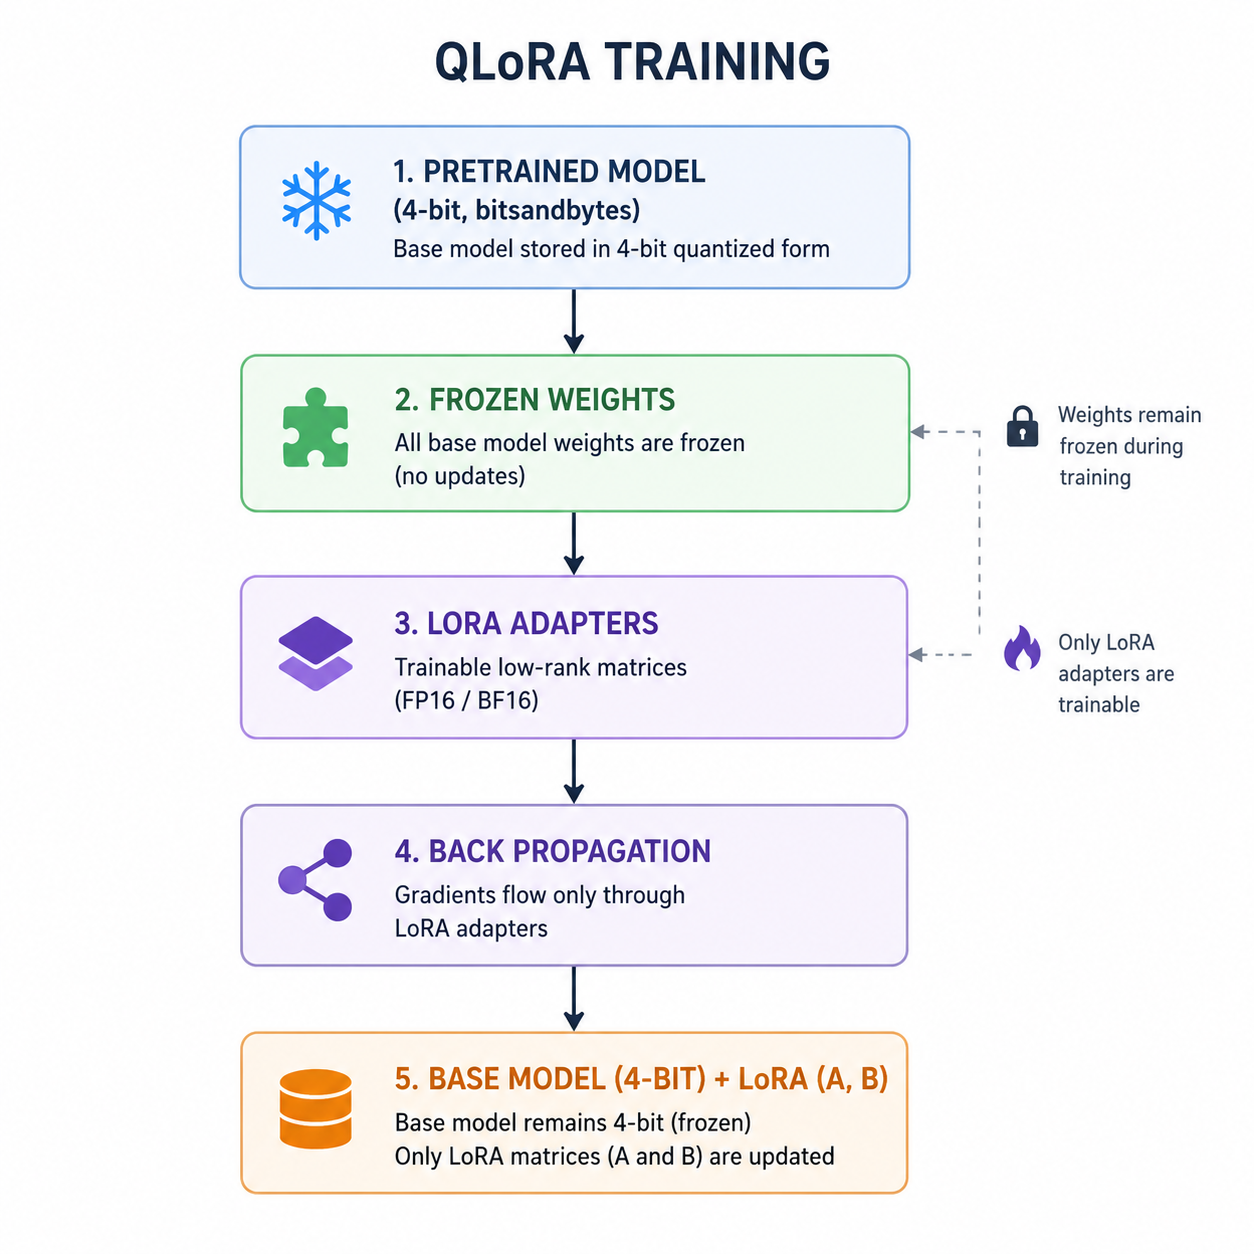
\includegraphics[width=0.85\textwidth]{figures/12-5 figure.png}
\end{figure}

Compared with standard LoRA, the only architectural difference is that the pretrained backbone is quantized before training.

\[
\boxed{
\text{4-bit Quantized Base Model (Frozen)}
+
\text{Trainable LoRA Adapters}
\longrightarrow
\text{Fine-Tuned Model}
}
\]

A common misconception is that QLoRA trains the quantized 4-bit weights. This is incorrect. The quantized backbone is used only during the forward computation and remains completely frozen throughout training. Backpropagation updates only the LoRA matrices ($A$ and $B$), exactly as in standard LoRA.

\subsection*{Key Innovations of QLoRA}

QLoRA combines LoRA with several techniques that make 4-bit fine-tuning practical.

\begin{enumerate}
    \item \textbf{NF4 (NormalFloat4)}\\
    Instead of using standard INT4 quantization, QLoRA adopts the NF4 numerical format, which is specifically designed for neural network weights. Since pretrained weights approximately follow a Gaussian distribution, NF4 represents them more accurately and reduces quantization error.

    \item \textbf{Double Quantization}\\
    Besides quantizing the model weights, QLoRA also quantizes the scaling factors used during quantization. This further reduces memory consumption with almost no loss in performance.

    \item \textbf{Paged Optimizers}\\
    GPU memory usage often fluctuates during training because optimizer states temporarily require additional memory. Paged optimizers dynamically move these temporary states between GPU and CPU memory, preventing memory spikes and enabling stable fine-tuning of much larger models.
\end{enumerate}

\subsection*{Advantages}

Compared with standard LoRA, QLoRA offers several important advantages:

\begin{itemize}
    \item Significantly lower GPU memory consumption.
    \item Fine-tuning of much larger language models on a single GPU.
    \item Performance comparable to full fine-tuning on many downstream tasks.
    \item Retains all advantages of LoRA while adding memory-efficient model storage.
\end{itemize}

Consequently, QLoRA has become one of the most influential techniques for parameter-efficient fine-tuning. By combining low-rank adaptation with 4-bit quantization, it enables high-quality fine-tuning of modern Large Language Models using affordable hardware.
\begin{table}[H]
\centering
\caption{Comparison of Full Fine-Tuning, LoRA, and QLoRA.}
\label{tab:ft_lora_qlora}

\renewcommand{\arraystretch}{1.35}

\begin{tabular}{|p{3.5cm}|p{2.8cm}|p{3.0cm}|p{2.6cm}|}
\hline
\rowcolor{gray!15}
\textbf{Method} &
\textbf{Base Model} &
\textbf{Trainable Parameters} &
\textbf{GPU Memory} \\
\hline

Full Fine-Tuning &
FP16 / BF16 &
All model parameters &
Very High \\
\hline

LoRA &
FP16 / BF16 &
Only LoRA matrices ($A$, $B$) &
Moderate \\
\hline

QLoRA &
4-bit (NF4) &
Only LoRA matrices ($A$, $B$) &
Low \\
\hline

\end{tabular}

\end{table}
\section*{Chapter Summary}

Modern Large Language Models contain billions of parameters, making full fine-tuning computationally expensive in terms of GPU memory, training time, and storage requirements. Parameter-Efficient Fine-Tuning (PEFT) addresses this challenge by freezing the pretrained backbone and training only a small number of additional parameters.

Among PEFT methods, LoRA has become the most widely adopted approach because it represents weight updates using low-rank matrices, dramatically reducing the number of trainable parameters while maintaining competitive performance.

QLoRA further extends this idea by storing the frozen backbone in 4-bit precision using NF4 quantization while continuing to train only the LoRA adapters. Combined with techniques such as Double Quantization and Paged Optimizers, QLoRA enables high-quality fine-tuning of very large language models on a single consumer GPU.

Today, LoRA and QLoRA have become the standard approaches for adapting modern Large Language Models because they provide an excellent balance between computational efficiency, memory usage, and downstream task performance.


\section{Beyond LoRA: Recent PEFT Methods}

Although LoRA and QLoRA have become the dominant approaches for parameter-efficient fine-tuning, numerous variants have been proposed to overcome some of their limitations. These methods generally aim to improve parameter allocation, optimization stability, memory efficiency, or adaptation capacity while preserving the fundamental PEFT philosophy of updating only a small subset of parameters.

Table~\ref{tab:modern_peft} summarizes some representative LoRA variants.
\begin{table}[H]
\centering
\caption{Representative extensions of LoRA.}
\label{tab:modern_peft}

\renewcommand{\arraystretch}{1.35}

\begin{tabular}{|p{2.6cm}|p{9cm}|}
\hline
\rowcolor{gray!15}
\textbf{Method} &
\textbf{Main Idea} \\
\hline

AdaLoRA &
Dynamically adjusts the rank of each layer during training, allocating more parameters to important layers and fewer to less important ones. \\
\hline

DoRA &
Separates each weight into magnitude and direction, allowing them to be optimized independently for improved stability and accuracy. \\
\hline

IA$^3$ &
Learns small scaling vectors that amplify or suppress activations instead of learning low-rank matrices, resulting in extremely low memory consumption. \\
\hline

LoRA+ &
Uses different learning rates for the LoRA matrices $A$ and $B$, leading to faster convergence and improved optimization. \\
\hline

VeRA &
Replaces most trainable matrices with fixed random matrices and learns only a small number of vectors, further reducing trainable parameters. \\
\hline

MoRA &
Improves the expressive power of low-rank adaptation by using richer matrix structures while remaining parameter efficient. \\
\hline

\end{tabular}

\end{table}
Despite these improvements, LoRA and QLoRA remain the most widely adopted PEFT techniques because they provide an excellent balance between simplicity, efficiency, and downstream performance. Most recent methods should therefore be viewed as refinements of LoRA rather than completely new fine-tuning paradigms.
\section{Practical PEFT Fine-Tuning Pipeline}

The practical workflow for fine-tuning a Large Language Model using LoRA or QLoRA typically consists of the following steps.
\subsection*{Step 1: Prepare the Dataset}

The first requirement is a task-specific dataset. Depending on the application, the dataset may contain:

\begin{itemize}
\item Question--Answer pairs
\item Instruction--Response pairs
\item Multi-turn conversations
\item Code and explanations
\item Translation examples
\item Summarization pairs
\end{itemize}

For example,

\begin{quote}
Instruction: Explain Newton's First Law.

Response: Newton's First Law states that...
\end{quote}

The objective is for the model to learn to generate the desired response.
\subsection*{Step 2: Format the Dataset}

Most LLM training frameworks expect structured datasets, typically stored in JSON or JSONL format.

\begin{verbatim}
{
  "instruction": "Translate to French",
  "input": "Hello",
  "output": "Bonjour"
}
\end{verbatim}

Different models may require slightly different dataset formats.
\subsection*{Step 3: Apply the Chat Template}

Modern instruction-tuned LLMs are trained using predefined conversation templates rather than raw text.

For example,

User:
What is Artificial Intelligence?

Assistant:
Artificial Intelligence is...

Each model family (Llama, Qwen, Gemma, Mistral, etc.) defines its own chat template, which must be used during training.
\subsection*{Step 4: Tokenization}

The formatted text is converted into token IDs using the tokenizer associated with the pretrained model.
\subsection*{Step 5: Configure LoRA or QLoRA}

Typical LoRA hyperparameters include

\begin{itemize}
\item Rank ($r$)
\item Scaling factor ($\alpha$)
\item Dropout
\item Target modules
\item Learning rate
\item Batch size
\item Number of epochs
\end{itemize}

When using QLoRA, additional settings include

\begin{itemize}
\item 4-bit loading
\item NF4 quantization
\item Compute data type (FP16 or BF16)
\end{itemize}
\subsection*{Step 6: Fine-Tuning}

Training follows the standard optimization pipeline

\[
\text{Input}
\rightarrow
\text{Forward Pass}
\rightarrow
\text{Loss}
\rightarrow
\text{Backpropagation}
\rightarrow
\text{Update LoRA Parameters}
\]

Only the adapter parameters are updated, while the pretrained backbone remains frozen.
\subsection*{Step 7: Evaluation}

The fine-tuned model is evaluated using metrics appropriate for the target task, such as

\begin{itemize}
\item Validation Loss
\item Accuracy
\item BLEU
\item ROUGE
\item Human Evaluation
\item Task-specific benchmarks
\end{itemize}
\subsection*{Step 8: Save the Adapter}

Instead of saving the entire LLM, only the LoRA adapter weights together with their configuration are stored.

This produces checkpoints that are dramatically smaller than the original pretrained model.
\subsection*{Step 9: Inference}

During deployment, the saved adapter is loaded together with the pretrained backbone.

Alternatively, the adapter can be merged permanently into the base model before inference.

Modern PEFT workflows are commonly implemented using libraries such as

\begin{itemize}
\item Hugging Face Transformers
\item PEFT
\item bitsandbytes
\item TRL
\item Datasets
\item Accelerate
\end{itemize}


\begin{figure}[H]
\centering
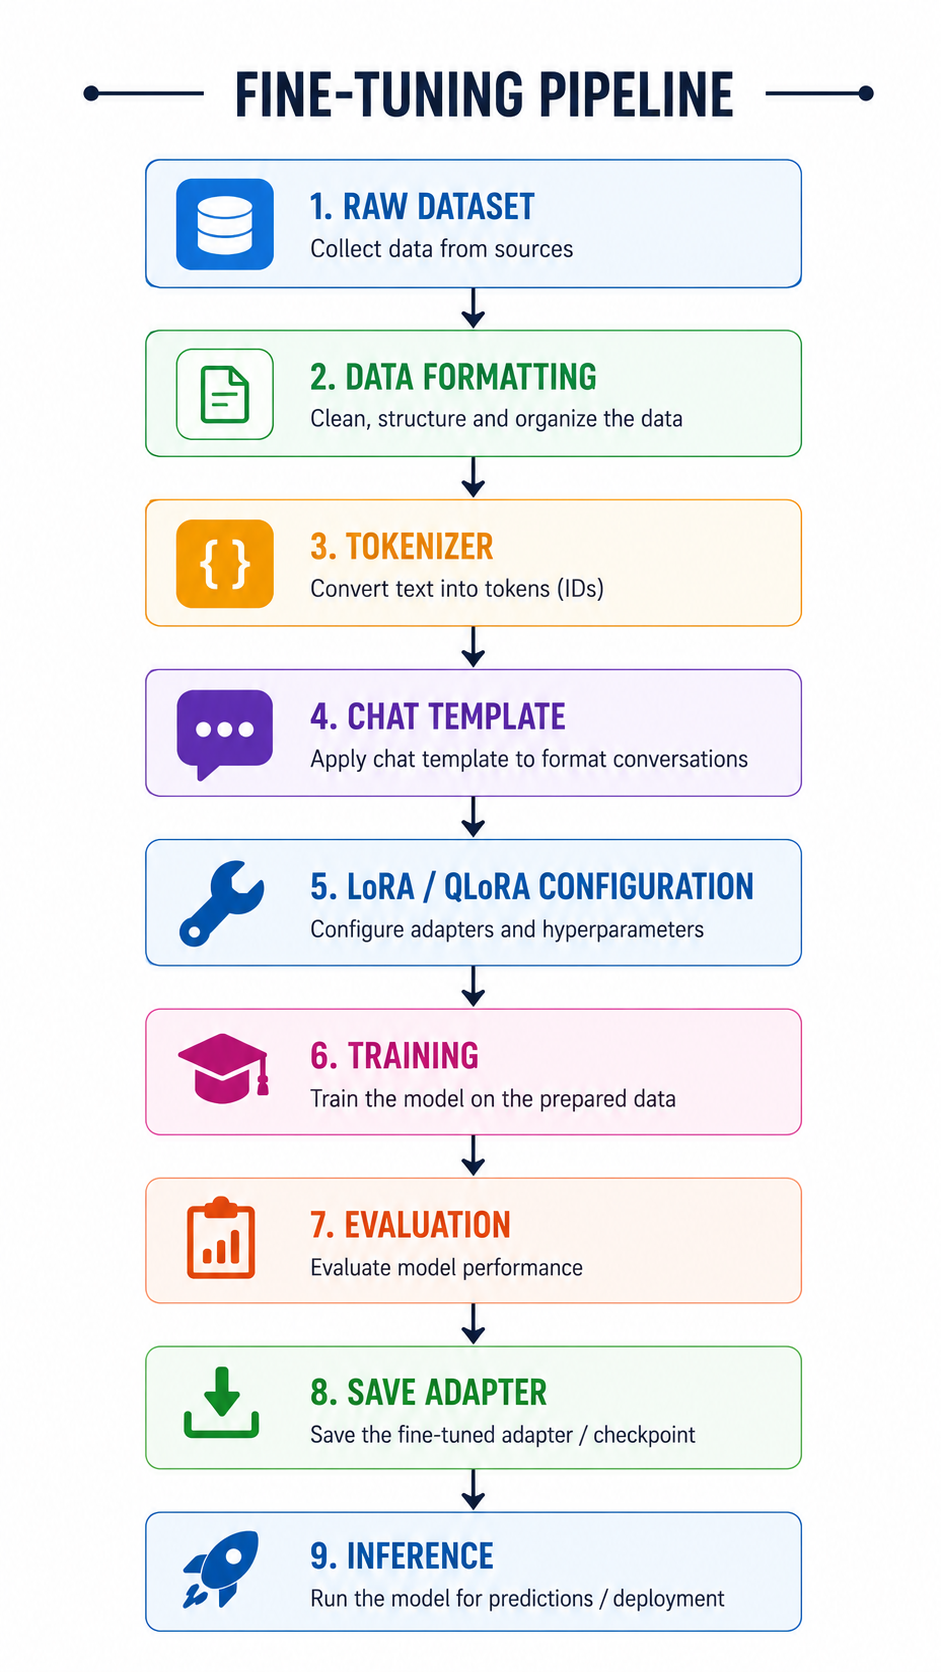
\includegraphics[width=0.85\textwidth]{figures/12-3 figure.png}
\end{figure}
